% Paper for CGAT
\documentclass[10pt, conference, compsocconf]{IEEEtran}

\usepackage{float}
%\usepackage{url}
\usepackage{graphicx}
\usepackage{subfig}
\usepackage{color}

\begin{document}

\title{CGAT In The Hat}

% author names and affiliations
% use a multiple column layout for up to two different
% affiliations

\author{\IEEEauthorblockN{Eriq Augustine, Ryan Hnarkis, Aldrin Montana, Ryan Verdon, Tyler Yero}
\\
\IEEEauthorblockA{Department of Computer Science\\
Cal Poly, San Luis Obispo\\
 \textsf{\{eaugusti, rhnaraki, amontana, rverdon, tyero\}@calpoly.edu}
}
}

\maketitle

\thispagestyle{empty}
\pagestyle{empty}

\section{Introduction}\label{sec:introduction}
Gene annotation is the process of associating metadata about a gene with the
contig, a dna sequence, on which the gene resides. This metadata is necessary for conducting
genomic research projects and analysis involving the contig's genomic sequence.
Currently, there is no specialty gene annotation software. Genome browsers
all maintain lots of genomic data and are used when manually annotating genes,
but do not provide a user-friendly interface. While genome browsers
will likely never be replaced (UCSC genome browser, etc. are well
established), it would be desirable to have a software system that better
accommodates the visual and informational needs of gene annotation.

\textit{CGAT} is a web-based gene annotation application designed with
usability, simplicity, and efficiency in mind. It is not a feature and data
rich genome browser like the \textit{UCSC genome brower}. Nor is \textit{CGAT}
designed to be a replacement for other genome browsers in any aspect other than
gene annotation. Other gene browsers attempt to accommodate many needs of the
biology community and so offer many features, and a cluttered, chaotic
interface. Gene annotation, while not a trivial task, can be well-serviced by a
simple data model. Ideally, by focusing on a simple data model, \textit{CGAT}
is able to provide a clean, streamlined experience. \textit{CGAT} aims to
provide users with a way to view gene annotations without extra, unnecessary
information obscuring their view while also embodying a Wikipedia-like emphasis
on collaboration and openness.

%Anya Goodman, a professor in the biochemistry department at Cal Poly, San Luis
%Obispo, offers a bioinformatics course that covers several aspects of gene
%annotation. This project is spearheaded by Ryan Verdon to accommodate Dr.
%Goodman's needs and ideas for ideal gene annotation software.

This paper primarily focuses on considerations for \textit{CGAT}s database
architecture. These considerations are made with regards to a MySQL cluster
versus a Couchbase cluster to determine which database architecture is most
efficient for running \textit{CGAT}. Section \ref{sec:motive} discusses our
motivation to compare Couchbase and MySQL in this paper, while section
\ref{sec:design} talks about how we designed experimental workloads to use for
our comparison of Couchbase vs MySQL. In section \ref{sec:workload} we
describe the workloads and how they are relevant to \textit{CGAT}, some brief
implementation details are outlined in section \ref{sec:implementation}, we
evaluate our results in section \ref{sec:eval} and finally conclude in
section \ref{sec:conclusions}.

\section{Motivation}\label{sec:motive}
Traditional web applications are almost always backed by a relational database.
However, there has been a recent movement towards the use of NoSQL databases for
web applications. Our main goal is to determine whether a NoSQL database, Couchbase,
can outperform a traditional relational database, MySQL, for \textit{CGAT}'s
common operations.

\section{Database Choice}
% TODO(ryan): Put decision and considereations here.
%  Schema will go in implementation section.
%  Incoude some text about how having the documents in JSON (Mongo is actually BSON) makes it really easy to use in JSON.

\section{Implementation}\label{sec:implementation}
CGAT uses a standard LAMP stack with MySQL traded out for MongoDB.

\subsection{Backend}
The \textit{backend} of the system consists of a PHP server connecting to a MongoDB database.
We do not use any templating systems.
We chose PHP for the backend because we did not require most of the functionality of a templating system, and we wanted a simple
system that can be easily understood when passed off to the next generation.

Mongo's PHP connecter is fully featured.
TODO(eriq): Cite mongo's php connector.

\subsubsection{Database Schema}

\subsubsection{API}
CGAT is an entireley API driven product. The API is central to all the behavior.
The API supplies \textbf{all} the information that is displayed in the UI.
This is a very important design choice. Having the API be the sole data provider and manipulator for the system
means that all functionality can be programatically provided and different applications can present the same
fuinctionality with a different UI.

The API accepts GET and PUT requests (depending on the action) and will always return a JSON response.

The current API supports 21 different calls, 7 GET requests and 14 POST actions.

\paragraph{GET Requests}
\begin{itemize}
\item administration_info - Provides the user with meta information information that the user would need to perform administrative tasks such as greating a group or assigning a task.
\item annotation - Provide the user with information about an specified annotation.
\item contig - Get information about a specific contig.
\item gene - Get information about a specific gene.
\item group - Get information about a specific group.
\item help - Get help information on a specific topic.
\item user_profile - Get the profile information about a specific user. If the user is logged in and requests information about themselves, more information is provided.
\end{itemize}

\paragraph{POST Actions}
Most POST actions require that the user is logged in.

\begin{itemize}
\item assign_task - Ask a group of people to perform an annotation.
\item cancel_notification - Clear a notification from a user.
\item create_annotation - Create a new annotation of a contig.
\item create_group - Create a group.
\item join_group - Join a group.
\item leave_group - Leave a group.
\item login - Login.
\item logout - Logout.
\item parse_fasta - Upload a FASTA file to the server, parse the contents, and returned the parsed structure.
\item register - Register a new user.
\item save_annotation - Save a work-in-progress annotation.
\item set_help - Upload a help page.
\item submit_annotation - Submit a finalized annotaion.
\item upload_contig - Uplaod a contig into CGAT.
\end{itemize}

\subsection{Frontend}

\section{UI Design}

\onecolumn
\appendices

\section{JSON Data Models}\label{sec:data_models}
\centering
Here are diagrams depicting our JSON data model.

\begin{figure*}[t]
   \centering
   \subfloat[Contig format]{\label{fig:JSON-contig}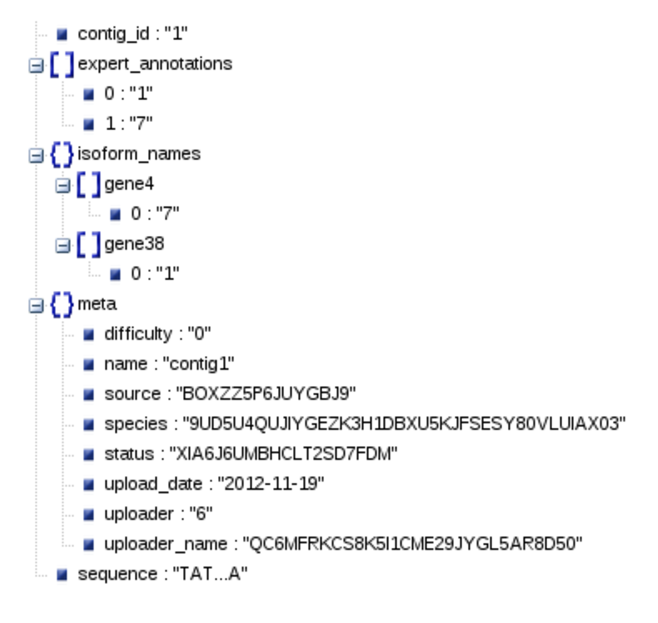
\includegraphics[height=70mm]{contig.eps}}
   \subfloat[Annotation format]{\label{fig:JSON-annotation}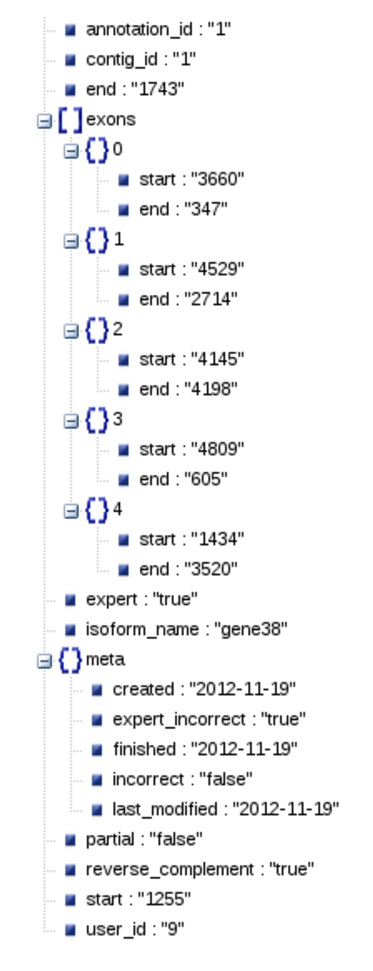
\includegraphics[height=80mm]{annotation.eps}}
   \caption{JSON format for Contigs and Annotations.}
\end{figure*}

\begin{figure*}[t]
   \centering
   \subfloat[User format]{\label{fig:JSON-user}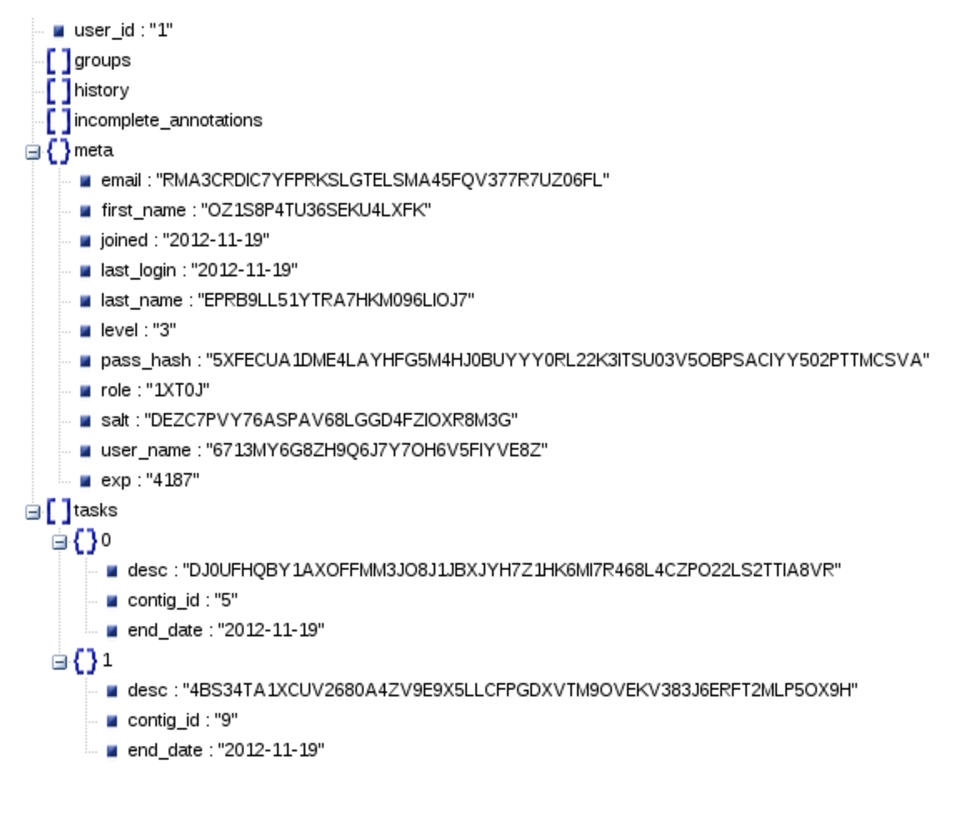
\includegraphics[height=90mm]{user.eps}}
   \subfloat[Group format]{\label{fig:JSON-group}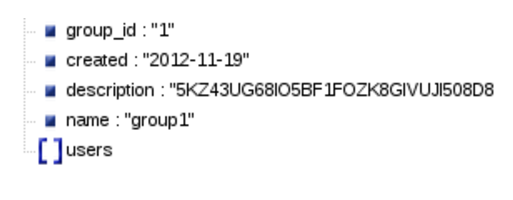
\includegraphics[height=25mm]{group.eps}}
   \caption{JSON format for Users and Groups.}
\end{figure*}

%\begin{figure*}
%  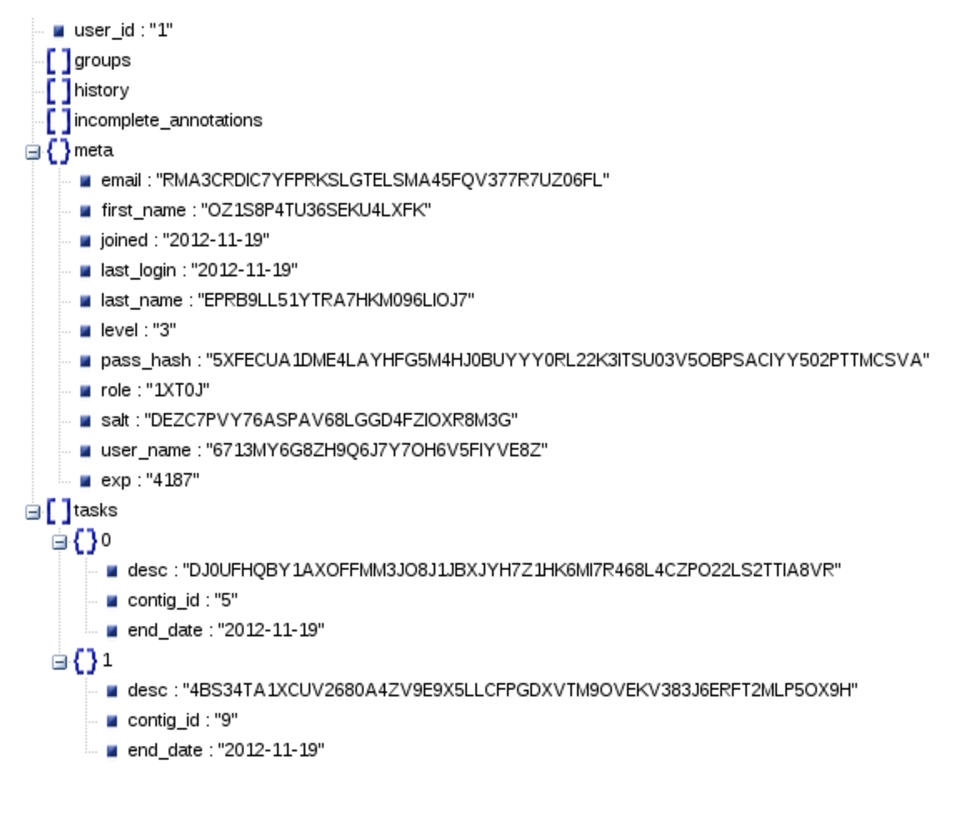
\includegraphics[height=90mm]{user.eps}
%	\caption{The JSON for a user.}
%	\label{fig:JSON-user}
%\end{figure*}
%\begin{figure*}
%  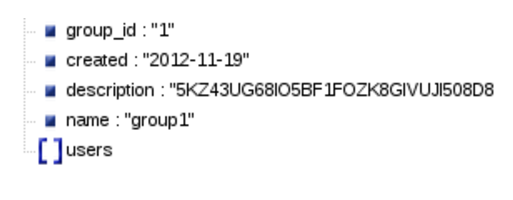
\includegraphics[height=25mm]{group.eps}
%	\caption{The JSON for a group.}
%	\label{fig:JSON-group}
%\end{figure*}
%\begin{figure*}
%  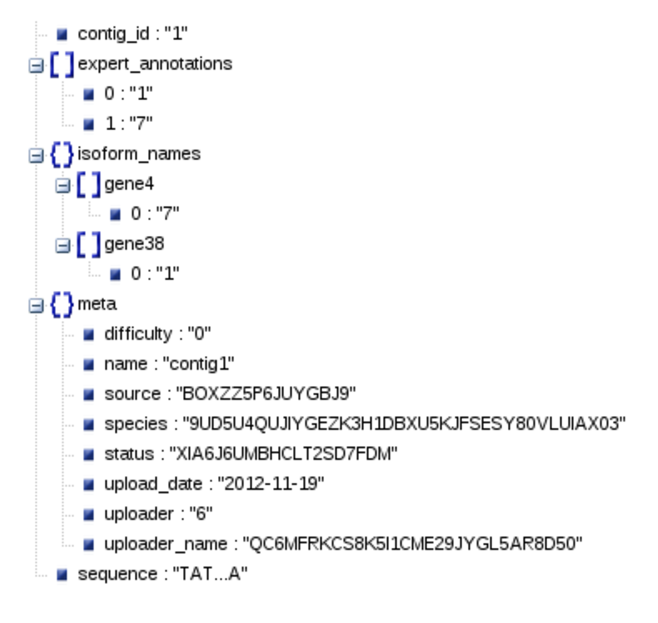
\includegraphics[height=80mm]{contig.eps}
%  \caption{The JSON for a contig.}
%  \label{fig:JSON-contig}
%\end{figure*}
%\begin{figure*}
%  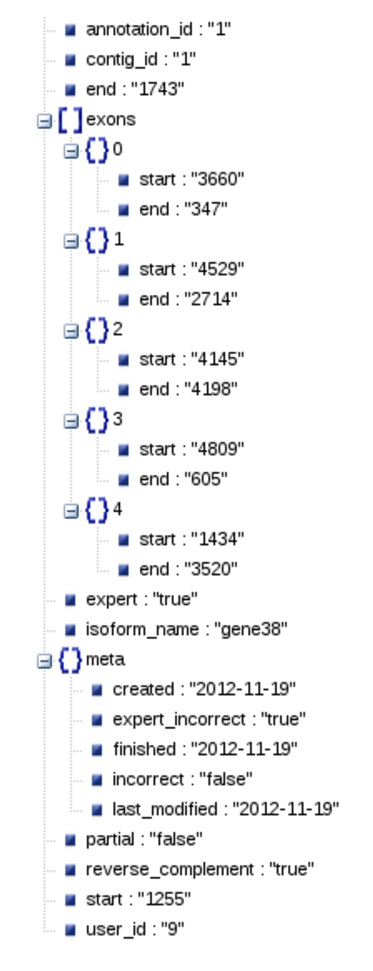
\includegraphics[height=90mm]{annotation.eps}
%	\caption{The JSON for an annotation.}
%	\label{fig:JSON-annotation}
%\end{figure*}

% TODO: Uncomment if we use any refs
% \bibliographystyle{acm}
% \bibliography{refs}

\end{document}
